% regression_experiment_proposal.tex
% Self-contained proposal/write-up of the sine-frequency regression experiment
% addressed by Decision 1 in decisions_needed.txt.
%
% Compile with: pdflatex regression_experiment_proposal.tex
% (twice, to resolve cross-references). No external .bib required.

\documentclass[11pt]{article}
\usepackage[margin=1in]{geometry}
\usepackage{amsmath,amssymb}
\usepackage{graphicx}
\usepackage{booktabs}
\usepackage{hyperref}
\usepackage{xcolor}

\title{Proposal: Sine-Frequency Regression as a Test of Prediction~4\\
{\large Standalone document for Decision~1 of the revision plan}}
\author{Gladwin Osakwe \and Nalini Ramanathan}
\date{}

\begin{document}
\maketitle

\section*{Purpose of this document}
This document is a self-contained proposal for the regression experiment
referenced in \texttt{decisions\_needed.txt}, Decision~1. It is \emph{not}
part of the main paper. Its purpose is to let the team decide whether the
sine-frequency regression sweep should be incorporated as a new
Section~3.5 (or new Section~4) of the manuscript. All experimental code
and outputs already exist in the repository
(\texttt{regression\_experiment.py},
\texttt{figures/heatmap\_depth\_vs\_ruggedness.png},
\texttt{figures/cosine\_sim\_Effect\_of\_Target\_Ruggedness\_on\_SG\_Alignment.png}).

\section{Motivation: Prediction~4 of the revision plan}
The revision plan introduces four predictions derived from the chain-rule
compounding mechanism. Prediction~4 states:
\begin{quote}
\itshape
Landscape ruggedness should have a secondary effect relative to depth,
because ruggedness affects the loss geometry but not the number of
surrogate approximations in the backpropagation chain.
\end{quote}
Without an experiment that varies ruggedness independently of depth, this
prediction is asserted but not tested. The classification setting used
elsewhere in the paper (\texttt{make\_moons}, \texttt{make\_circles})
varies ruggedness only weakly between datasets. We need a knob that
moves landscape ruggedness over a wide range while holding architecture
and dataset family fixed.

\section{Method}
\paragraph{Task.} A 1D regression problem where the target is a sum of
random sine waves:
\[
y(x) \;=\; \frac{1}{K}\sum_{k=1}^{K} a_k\,\sin(f_k\,x + \phi_k),\qquad
x \sim \mathrm{Uniform}(-2,\,2),
\]
with $K \in \{1,3,5,10\}$. Frequencies $f_k\sim\mathrm{Uniform}(2,15)$,
phases $\phi_k\sim\mathrm{Uniform}(0,2\pi)$, amplitudes
$a_k\sim\mathrm{Uniform}(0.5,1.5)$ are drawn once per ruggedness level
and held fixed across architectures. Normalisation by $K$ keeps the
output range comparable across $K$. The number of frequencies $K$
controls landscape ruggedness in a controlled way: $K=1$ gives a smooth
near-quadratic loss; $K=10$ gives a highly non-convex landscape with
many local minima.

\paragraph{Architecture and optimisation.} Identical to the classification
setup elsewhere in the paper: sigmoid-activation MLPs, hidden width 64,
$\beta_f = 50$, $\beta_{\mathrm{sg}} = 5$, full-batch SGD, $\mathrm{lr}=0.01$,
$500$ epochs, MSE loss. The depth axis is swept over
$L \in \{1,2,3,4\}$, giving a $4 \times 4$ depth-by-ruggedness grid.

\paragraph{Twin-network protocol.} The twin-network setup of Section~2.1
of the main paper is reused: \textsc{MLP-true} and \textsc{MLP-surrogate}
share weights at every step, so the only difference between their
gradients is the activation derivative used in backprop.

\paragraph{Metric.} Per-cell scalar is the mean cosine similarity between
$g_{\mathrm{sg}}$ and $g_{\mathrm{true}}$ over the last 50 epochs, matching
the convention in Section~3.

\section{Result (already produced)}
Figure~\ref{fig:heatmap} shows the $4\times4$ heatmap. The axes are
hidden-layer depth (rows) and number of frequencies $K$ (columns). The
qualitative finding directly supports Prediction~4: cosine similarity
falls sharply with depth across every column, while moving along the
ruggedness axis at fixed depth produces a much smaller change. Depth
dominates ruggedness, exactly as Prediction~4 anticipates.

\begin{figure}[h]
  \centering
  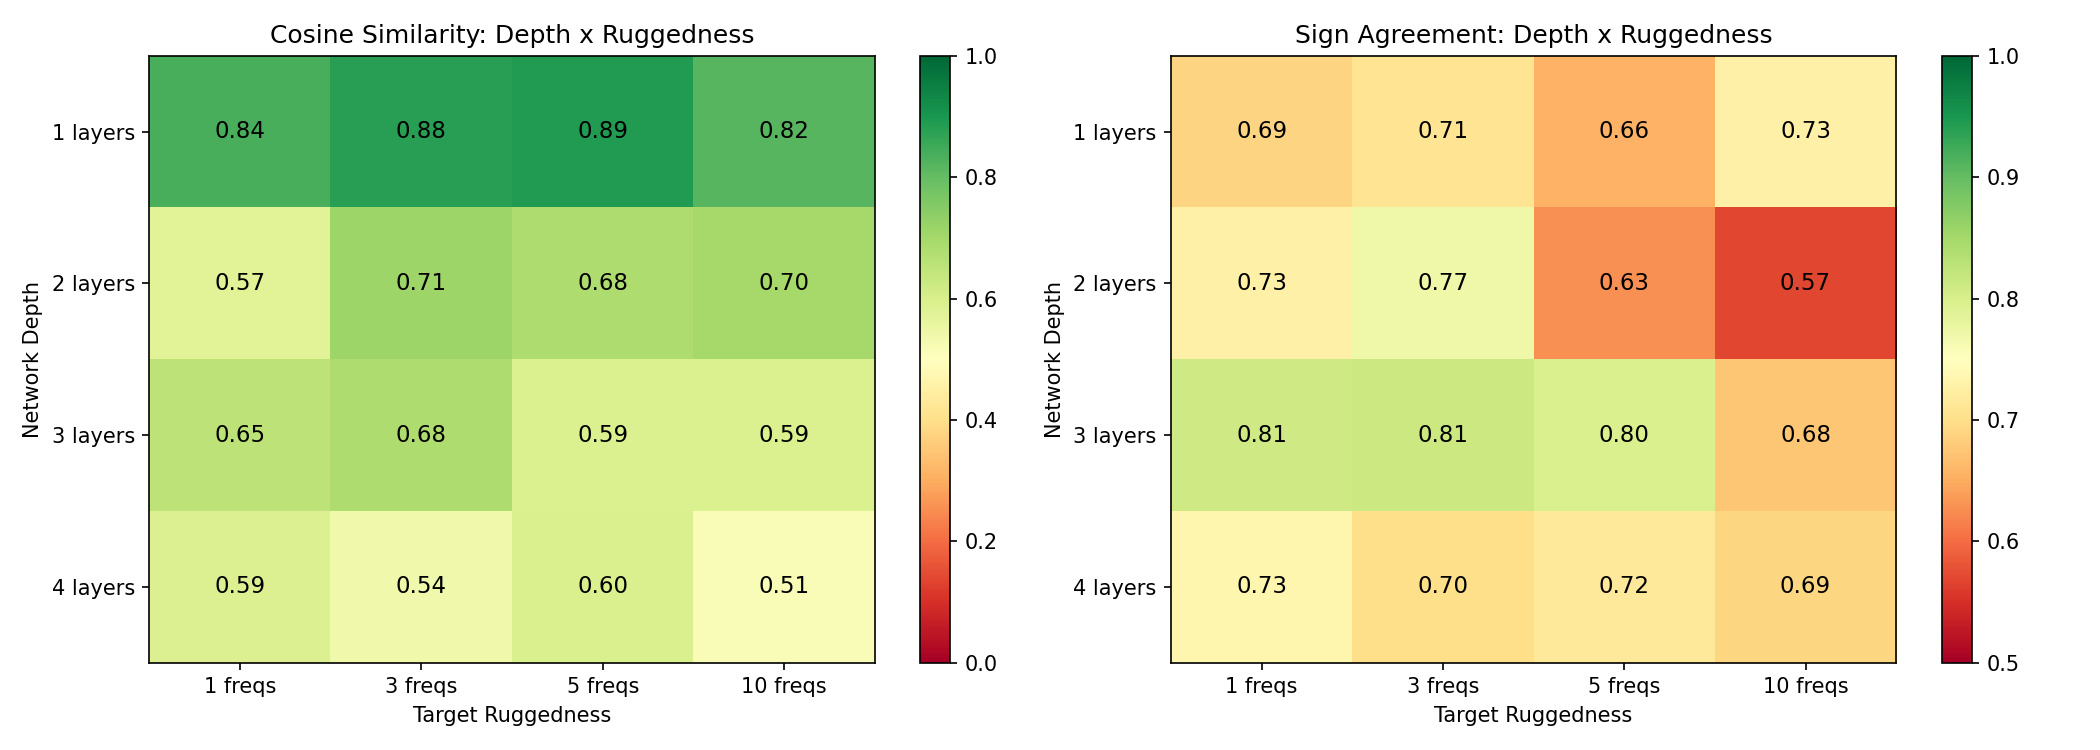
\includegraphics[width=0.85\linewidth]{figures/heatmap_depth_vs_ruggedness.png}
  \caption{Depth-by-ruggedness heatmap of mean cosine similarity (last
  50 epochs). Rows: hidden-layer depth $L\in\{1,2,3,4\}$. Columns:
  number of sine components $K\in\{1,3,5,10\}$ (left = smooth, right =
  rugged). Dropping vertically (depth) changes the metric far more than
  moving horizontally (ruggedness), supporting Prediction~4.}
  \label{fig:heatmap}
\end{figure}

A complementary line plot --- cosine similarity over training for fixed
depth $L=3$ across the four ruggedness levels --- is available in
\texttt{figures/cosine\_sim\_Effect\_of\_Target\_Ruggedness\_on\_SG\_Alignment.png}.

\section{Recommended placement in the manuscript}
Two options:
\begin{description}
\item[Option A: new Section~3.5.] Append immediately after the
  capacity-controlled depth sweep, framed as ``ruggedness as a control
  for depth''. Lowest disruption to the existing structure; the heatmap
  fits as one figure and the result paragraph is roughly half a page.
\item[Option B: new Section~4 (renumbering downstream).] Promote to a
  standalone short section titled ``Ruggedness vs.~depth'' between the
  current Sections~3 and~4. Slightly more visible, but forces
  renumbering of the late-training collapse and per-layer sections.
\end{description}
We recommend \textbf{Option A}: lower editing cost and the result
naturally completes the depth-effect arc of Section~3.

\section{Required edits if accepted}
\begin{enumerate}
  \item Insert a $\sim$1-page subsection (Section~3.5 or Section~4) with
        the figure, the four-paragraph write-up sketched above, and a
        single sentence linking back to Prediction~4
        (Section~\texttt{sec:predictions}).
  \item Add one sentence to the abstract and one sentence to the
        Theoretical Predictions paragraph of Section~2 referencing the
        ruggedness experiment (this is Decision~2 in
        \texttt{decisions\_needed.txt}).
  \item No new bibliography entries are needed.
\end{enumerate}

\section{Reproducibility}
The experiment is already implemented and committed:
\begin{itemize}
  \item Code: \texttt{regression\_experiment.py} (two sweeps:
    ruggedness-only at $L=3$, and the full $4\times4$ interaction grid).
  \item Output figures: \texttt{figures/heatmap\_depth\_vs\_ruggedness.png}
    and the per-ruggedness line plot named above.
  \item No re-running is needed to support the proposed subsection;
    the existing artifacts are sufficient.
\end{itemize}

\end{document}
